% Guides
% http://ivk.knteu.kiev.ua/docum/z_vg.pdf
% http://www.ivk.knteu.kiev.ua/docum/prav01.pdf
\documentclass[a4paper,14pt,oneside,final]{extarticle}
\usepackage[top=2cm, bottom=2cm, left=3cm, right=1cm]{geometry}
\usepackage{scrextend}

\usepackage[T2A,T1]{fontenc}
\usepackage[ukrainian,russian,english]{babel}
\usepackage{tempora}
\usepackage{fontspec}
\setmainfont{tempora}

% Зачем: Отключает использование изменяемых межсловных пробелов.
% Почему: Так не принято делать в текстах на русском языке.
\frenchspacing

\usepackage{indentfirst}
\setlength{\parindent}{1.25cm}
\renewcommand{\baselinestretch}{1.5}

% Header
\usepackage{fancyhdr}
\pagestyle{fancy}
\fancyhead{}
\fancyfoot{}
\fancyhead[R]{\small \selectfont \thepage}
\renewcommand{\headrulewidth}{0pt}

% Captions
\usepackage{chngcntr}
\counterwithin{figure}{section}
\counterwithin{table}{section}
\usepackage[tableposition=top]{caption}
\usepackage{subcaption}
\DeclareCaptionLabelFormat{gostfigure}{Рисунок #2}
\DeclareCaptionLabelFormat{gosttable}{Таблиця #2}
\DeclareCaptionLabelSeparator{gost}{~---~}
\captionsetup{labelsep=gost}
\captionsetup[figure]{labelformat=gostfigure}
\captionsetup[table]{labelformat=gosttable}
\renewcommand{\thesubfigure}{\asbuk{subfigure}}

% Sections
\usepackage[explicit]{titlesec}
\newcommand{\sectionbreak}{\clearpage}

\titleformat{\section}
  {\centering}{\thesection \quad}{0pt}{\MakeUppercase{#1}}
\titleformat{\subsection}[block]
  {\bfseries}{\thesubsection \quad #1}{0cm}{}

\titlespacing{\section} {0cm}{0cm}{21pt}
\titlespacing{\subsection} {\parindent}{21pt}{0cm}
\titlespacing{\subsubsection} {\parindent}{0cm}{0cm}

% Lists
\usepackage{enumitem}
\renewcommand\labelitemi{--}
\setlist[itemize]{noitemsep, topsep=0pt, wide}
\setlist[enumerate]{noitemsep, topsep=0pt, wide, label=\arabic*}
\setlist[description]{labelsep=0pt, noitemsep, topsep=0pt, leftmargin=2\parindent, labelindent=\parindent, labelwidth=\parindent, font=\normalfont}

% Toc
\usepackage{tocloft}
\tocloftpagestyle{fancy}
\renewcommand{\cfttoctitlefont}{}
\setlength{\cftbeforesecskip}{0pt}
\renewcommand{\cftsecfont}{}
\renewcommand{\cftsecpagefont}{}
\renewcommand{\cftsecleader}{\cftdotfill{\cftdotsep}}

\usepackage{float}
\usepackage{pgfplots}
\usepackage{graphicx}
\usepackage{multirow}
\usepackage{amssymb,amsfonts,amsmath,amsthm}
\usepackage{csquotes}

\usepackage{listings}
\lstset{basicstyle=\footnotesize\ttfamily,breaklines=true}
\lstset{language=Matlab}

\usepackage[
	backend=biber,
	sorting=none,
	language=auto,
	autolang=other
]{biblatex}
\DeclareFieldFormat{labelnumberwidth}{#1}


\usepackage{lastpage}
\usepackage{calc}
\usepackage{soul}
\usepackage{pbox}
\usepackage{ulem}
\usepackage{titling}
\usepackage{framed}
\usepackage{tabu}
\usepackage{appendix}
\usepackage{packages/tikz-uml}
\usepackage[nomain,acronym,toc,nogroupskip,xindy={glsnumbers=false}]{glossaries}
\usepackage[figure,table]{totalcount}

\makeglossaries
\newglossarystyle{mylist}{%  
 % put the glossary in the itemize environment:  
 \renewenvironment{theglossary}%  
   {\begin{itemize}[label={}]}{\end{itemize}}%  
 % have nothing after \begin{theglossary}:  
 \renewcommand*{\glossaryheader}{}%  
 % have nothing between glossary groups:  
 \renewcommand*{\glsgroupheading}[1]{}%  
 \renewcommand*{\glsgroupskip}{}%  
 % set how each entry should appear:  
 \renewcommand*{\glossentry}[2]{%  
 \item % bullet point  
 \glstarget{##1}{\glossentryname{##1}}% the entry name  
 \space ---% the symbol in brackets  
 \space \glossentrydesc{##1}% the description  
 \space [##2]% the number list in square brackets  
 }%  
 % set how sub-entries appear:  
 \renewcommand*{\subglossentry}[3]{%  
   \glossentry{##2}{##3}}%  
 } 
\setglossarystyle{mylist}
 
\graphicspath{{figures/}}
\addbibresource{bibliography.bib}

\newacronym{am}{АМ}{агентне моделювання}
\newacronym{gis}{ГІС}{геоінформаційна система}
\newacronym{computer}{ЕОМ}{електронна обчислювальна машина}
\newacronym{mas}{МАС}{мультиагентна система}
\newacronym{pc}{ПЕОМ}{персональна електронна обчислювальна машина}
\newacronym{sw}{ПЗ}{програмне забезпечення}
\newacronym{smw}{СУОП}{система управління охороною праці}

%\newacronym{afapl}{AFAPL}{Agent Factory Agent Programming Language}
%\newacronym{api}{API}{Application Programming Interface}
%\newacronym{corba}{CORBA}{Common Object Request Broker Architecture}
%\newacronym{fipa}{FIPA}{Foundation for Intelligent Physical Agents}
%\newacronym{faq}{FAQ}{Frequently Asked Questions}
%\newacronym{lgpl}{LGPL}{GNU Lesser General Public License}
%\newacronym{gui}{GUI}{Graphical User Interface}
%\newacronym{jade}{JADE}{Java Agent Development Framework}
%\newacronym{jre}{JRE}{Java Runtime Environment}
%\newacronym{jvm}{JVM}{Java Virtual Machine}
%\newacronym{json}{JSON}{JavaScript Object Notation}
%\newacronym{uml}{UML}{Unified Modeling Language}

\newcommand{\khpistudentgroup}{КН-34г}
\newcommand{\khpistudentname}{Чепурний~А.~С.}

\newcommand{\khpidepartment}{Програмна інженерія та інформаційні технології управління}
\newcommand{\khpititlewhat}{
	Лабораторна робота №\labnumber \\
	з предмету <<Моделювання систем>>
}
\newcommand{\khpititlewho}{
	Виконав: \\
	\hspace*{\parindent} ст. групи \khpistudentgroup \\
	\hspace*{\parindent} \khpistudentname \\
	Перевірила: \\
	\hspace*{\parindent} ст. в. каф. ПІІТУ \\
	\hspace*{\parindent} Єршова~С.~І. \\
	\hspace*{\parindent} ас. каф. ПІІТУ \\
	\hspace*{\parindent} Литвинова~Ю.~С. \\
}


\begin{document}
\Ukrainian

\addtocounter{page}{4}
\renewcommand\contentsname{\hspace*{\fill}\bfseries\MakeUppercase{Зміст}\hspace*{\fill}}
\tableofcontents

\printglossary[type=\acronymtype,title={Перелік позначень та скорочень}]

\section*{Вступ}
\addcontentsline{toc}{section}{Вступ}

%Керуючись життєвим досвідом і науковими знаннями, людина будує моделі --- від паперових корабликів до картини світу. 
%Чим вони багатші і чим точніше ми можемо ними оперувати, тим краще наша свідомість --- наша <<найважливіша модель>>, відповідає реальності і знаходить способи її зміни.

% NaUKMAkn_2013_151_16.pdf
% http://www.economy.in.ua/pdf/1_2016/9.pdf
На сучасному етапі розвитку складні логістичні системи вимушені працювати в умовах високої невизначеності, що суттєво ускладнює управління ними. 
В процесі прийняття управлінських рішень виникає проблема прогнозування поведінки системи та зовнішнього середовища. 
Результати прогнозів необхідно постійно коригувати по ходу розвитку подій, що дозволяє пристосовуватися до змін оточення та гнучко реагувати на негативні впливи. 

У нагоді тут стає агентне моделювання, яке сягає своїм історичним корінням складних адаптивних систем і принципу побудови систем знизу вгору.
Агентне моделювання дозволяє здійснити множину прогнозів за різними сценаріями залежно від формування різноманітних ситуацій практично необмеженої складності. 

Основними елементами агентного моделювання є агенти, стосунки між ними і простір, в якому відбувається взаємодія. 
Агенти моделюються індивідуально. 
Вони можуть мати неповну інформацію, здійснювати помилки, адаптуватися до ситуації, проявляти ініціативу. 
В основу агентного моделювання закладені такі принципи, як різноманітність, взаємозв’язок і міра взаємодії. 
Тип взаємодій різних агентів може відрізнятися і носити ймовірнісний характер. 
Результатом динамічної взаємодії може бути певний рівноважний стан системи, а може бути і нова якість, яку неможливо передбачати з аналізу окремих складових системи.

Об'єктом дослідження є процес прийняття рішень розподільчою логістичною системою. 

Предметом дослідження є мультиагентна модель розподільчої логістичною системи. 

Теоретико-методологічною основою роботи є агентне моделювання, системний аналіз, а також базова теорія логістики.

Метою і завданням дослідження є розробка мультиагентної системи для дослідження розподільчої логістичної системи.
Для досягнення поставленої мети в курсовій роботі були сформульовані та вирішені наступні задачі:
\begin{itemize}
	% logistics
	\item описати динаміку розподільчої логістичної системи;
	\item дослідити проблеми імітаційного моделювання розподільчої логістичної системи;
	% agents
	\item порівняти фреймворки для реалізації мультиагентних систем, обрати та обґрунтувати вибір фреймворку;
	\item розробити специфікацію мультиагентної системи;
	\item реалізувати мультиагентну систему;
	\item верифікувати розроблену мультиагентну систему;
	\item протестувати мультиагентну систему на реальних даних;
	\item викласти пропозиції щодо перспектив розвитку та удосконалення розробленої мультиагентної системи.
\end{itemize}

%\section{Аналіз існуючих моделей і алгоритмів управління логістичними системами. Постановка задачі}
\section{Аналіз предметної області}
\subsection{Розподільча логістична система як об'єкт дослідження}
% https://essuir.sumdu.edu.ua/bitstream/123456789/38038/1/Bilovodska_Kyslyi_Olefirenko_Solyanyk.pdf
Розподільча логістика --- це частина загальної логістичної системи, яка забезпечує найбільш ефективну організацію розподілу продукції, охоплюючи систему товароруху і виконуючи логістичні операції транспортування, складування, упакування та ін.~\cite{Kusluy2010}.

Розподільча логістика спрямована на комплексне планування, управління та фізичне опрацювання потоку готових виробів у супроводі необхідного інформаційного, фінансового та сервісного потоку від моменту здачі-приймання товарів з виробництва до замовника (споживача) з метою оптимізації витратних та часових характеристик зазначеної частини матеріального і нематеріального потоків.
Головна мета розподільчої логістики --- організація розподільчої діяльності відповідно до замовлень клієнтів з мінімальними загальними витратами~\cite{Kusluy2010}.

Принципова відмінність розподільчої логістики від традиційного розуміння збуту полягає насамперед у системному взаємозв'язку процесу розподілу з процесами виробництва і закупівель під час управління матеріальними потоками, а також системному взаємозв'язку всіх функцій всередині самого розподілу.

Матеріальний потік у сфері розподілу має форму готової продукції.
Залежно від суб'єкту економічних відносин, який бере участь у доведенні ресурсів до споживача, потік готової продукції можна подати як товарний потік або як вантажний потік (на транспорті).

Розподільча логістика будується на загальних логістичних принципах~\cite{Anikin1999}:
\begin{itemize}
	\item координація всіх процесів товароруху, починаючи від кінцевих операцій товаровиробника та закінчуючи сервісом споживача;
	\item інтеграція всіх функцій управління процесами розподілу готової продукції та послуг, починаючи від визначення мети та закінчуючи контролем;
	\item адаптація комерційного, канального та фізичного розподілу до постійно змінних вимог ринку та потреб споживача;
	\item координація всіх процесів товароруху, починаючи від кінцевих операцій товаровиробника та закінчуючи сервісом споживача;
	\item системність як управління розподілом в його цілісності та взаємозалежності всіх елементів збутової діяльності;
	\item комплексність, тобто вирішення всієї сукупності проблем, пов’язаних із задоволенням платоспроможного попиту покупців;
	\item оптимальність стосовно як елементів системи, так і режиму її функціонування;
	\item раціональність як в організаційній структурі, так і в організації управління.
\end{itemize}

Склад завдань розподільчої логістики на мікро- та на макрорівні різний~(таблиця~\ref{tab:logistic_functions}). 

\begin{table}[H]
	\caption{Завдання розподільчої логістики на мікро- та макрорівнях}
	\label{tab:logistic_functions}
	\begin{tabular}{@{}|p{0.53\linewidth}|p{0.4\linewidth}|@{}}
	 	\hline
		Мікрорівень & Макрорівень \\ \hline
		\begin{itemize}[leftmargin=*]
			\item оптимізація формування портфеля замовлень;
			\item укладання договорів із замовниками на постачання продукції;
			\item забезпечення ритмічності та дотримання планомірності реалізації продукції;
			\item вивчення і задоволення потреб у логістичному сервісі;
			\item раціоналізація параметрів, структури і просування динамічних матеріальних потоків;
			\item оптимізація параметрів і умов зберігання запасів товарного характеру;
			\item формування і вдосконалення системи інформаційного забезпечення.
		\end{itemize}
		&
		\begin{itemize}[leftmargin=*]
			\item вибір схеми розподілу матеріального потоку;
			\item визначення оптимальної кількості розподільчих центрів на території, яка обслуговується;
			\item визначення оптимального місця розташування розподільчого центру на території, яка обслуговується, та ін.
		\end{itemize} \\ \hline
	\end{tabular}
\end{table}

\subsection{Проблеми моделювання і управління розподільчими логістичними системами}
Основною проблемою, характерною для об'єкта дослідження, яка породжує безліч інших проблем, є його ієрархічність і розподіленість. 
В таких системах процеси розосереджені по окремих підсистемах і знаходяться на різних рівнях ієрархії. 
Для таких систем вирішується комплекс взаємопов'язаних задач в режимі багатосторонньої взаємодії між менеджерами-аналітиками, що відповідають за окремі локальні завдання і \acrshort{computer}. 
Основними ознаками розподіленості будь-якої логістичної системи можна вважати:
\begin{itemize}
	\item наявність механізму розбиття даної системи на окремі взаємопов'язані підсистеми;
	\item окремі складові системи географічно відокремлені;
	\item відносна автономність окремих підсистем;
	\item спільне завдання всієї системи розглядається у вигляді набору окремих локальних підзадач;
	\item паралельність і асинхронність рішення окремих локальних задач різними виконавцями.
\end{itemize}

Першою проблемою, яку необхідно вирішувати, є розбиття кожної системи на окремі локальні підсистеми. 
Можна сказати, що формалізація цих двох завдань здійснюється на основі декомпозиції і агрегування. 
Декомпозиція полягає в розчленуванні вихідної задачі на ряд відносно незалежних підзадач, а агрегування --- в заміні окремих груп змінних, що характеризують ефективність функціонування системи, змінними-агрегатами. 
При цьому висувається вимога повної (достатньої) еквівалентності задач. 
Агрегування параметрів і змінних здійснюється в ході руху вгору по ієрархії. 
Це пов'язано з великою розмірністю завдання і неможливістю прийняття рішень на основі варіювання всіх параметрів і змінних. 
Основні ідеї, які реалізуються при синтезі моделі на основі декомпозиції і агрегування полягають у наступному:
\begin{itemize}
\item нехтуючи слабкими зв'язками між окремими підсистемами, зробити декомпозицію;
\item використовуючи трохи відмінності між ними, зробити агрегування;
\item використовуючи сильні відмінності, виділити <<вузькі місця>>, відкинувши на основі апріорних оцінок несуттєві обмеження.
\end{itemize}

\subsection{Моделі логістичних систем}
Моделювання в загальному вигляді являє собою один з основних методів пізнання, є формою відображення дійсності і полягає у з'ясуванні або відтворенні тих чи інших властивостей реальних об'єктів, процесів, явищ за допомогою абстрактного опису у вигляді зображення, плану, карти, сукупності рівнянь, алгоритмі і програм.

Одним з найбільш ефективних методів дослідження складних систем розподільчої логістики є імітаційне моделювання~\cite{Kobelev2003}.

Імітаційне моделювання --- експериментальний метод дослідження реальної системи за її імітаційною моделлю, який поєднує особливості експериментального підходу і специфічні умови використання обчислювальної техніки~\cite{Emelyanov2002}.

Серед переваг імітаційного моделювання відзначають~\cite{Emelyanov2002}: 
\begin{enumerate}
	\item Відображення динамічних процесів і поведінкових аспектів зовнішнього середовища.
	\item Можливість виявлення закономірностей, динамічних тенденцій розвитку і функціонування складної системи в умовах неповної та неточної інформації.
	\item Опис взаємодії та поведінки безлічі активних агентів в соціальних системах.
	\item Реалізацію принципів об'єктно-орієнтованого проектування і застосування високотехнологічних рішень при побудові комп'ютерних моделей та ін.
\end{enumerate}

Головною проблемою при побудові будь імітаційної моделі є необхідність побудови комплексних математичних моделей і розробки програмного коду імітаційної моделі. 

У імітаційному моделюванні виділяють такі основні підходи:
\begin{itemize}
	\item системна динаміка;
	\item дискретне моделювання;
	\item агентне моделювання.
\end{itemize}

\subsubsection{Системна динаміка}
Як методологія системна динаміка була запропонована в 1961 році Дж. Форрестером в якості інструменту дослідження інформаційних зворотних зв'язків у виробничо-господарської діяльності. 
Процеси, що відбуваються в реальному світі, в системній динаміці представляються в термінах накопичувачів і потоків між ними.
Системнодинамічна модель описує поведінку системи та її структуру як безліч взаємодіючих зворотних зв'язків і затримок. 
Математично така модель виглядає як система диференціальних рівнянь. 
Результатом моделювання в системній динаміці є виявлення глобальних залежностей і причинно-наслідкових зв'язків у досліджуваній системі~\cite{Shamrin2016}. 

\subsubsection{Дискретне моделювання}
Основний об'єкт в системі дискретного моделювання --- пасивний транзакт, який може певним чином представляти собою працівників, деталі, сировину, документи, сигнали і т. п.
Переміщаючись по моделі, транзакти стають в черги до одноканальним і багатоканальним пристроям, захоплюють і звільняють їх, розщеплюються, знищуються і т. д.
Відмінною особливістю даного підходу є час просування по моделі: або від події до події, або через дискретні проміжки часу. 
Дискретне моделювання застосовується, якщо можливо припустити, що змінні в системі змінюються миттєво в певні проміжки часу. 
Даний підхід імітаційного моделювання є одним з найпоширеніших і застосовується для дослідження соціально-економічних, технічних, логістичних та інших процесів.
На основі дискретного підходу реалізовано найбільше
число систем імітаційного моделювання~\cite{Shamrin2016}. 

\subsubsection{Агентне моделювання}
Агентське моделювання з'явилося в 90-х роках і використовується для дослідження децентралізованих систем, динаміка функціонування яких визначається не глобальними правилами і законами (як в інших парадигмах моделювання), а коли ці глобальні правила і закони є результатом індивідуальної активності членів групи.

Агентно-орієнтована система може складатися з одного агента (наприклад, програмний секретар~\cite{Maes1995}), проте весь потенціал розкривається з використанням мультиагентної системи~\cite{Waters1989}.
Під агентом розуміється система, яка має такі властивості~\cite{Jennings1998,Wooldridge1995}:
\begin{enumerate}[label={\arabic*)}]
	\item автономність: агенти мають внутрішній стан (який недоступний іншим агентам) та приймають рішення на основі своїх даних, без прямого втручання людини;
	\item реактивність: агенти розміщуються в навколишньому середовищі (яке може бути фізичним світом, множиною інших агентів, інтернетом і т.д.), здатні спостерігати і своєчасно реагувати на зміни;
	\item проактивність: агенти не тільки реагують на зміни в зовнішньому середовищі, вони здатні виявляти ініціативу для досягнення своєї мети;
	\item соціальність: агенти взаємодіють з іншими агентами (і, можливо, людиною) через спеціальний інтерфейс для досягнення їх цілей.
\end{enumerate}

Мета агентських моделей --- отримати уявлення про ці глобальні правила, загальну поведінку системи, виходячи з припущень про індивідуальну, приватну поведінку її окремих активних об'єктів і взаємодію цих об'єктів в системі.
У разі моделювання логістичних систем, що містять великі кількості активних об'єктів (людей, машин, підприємств чи навіть проектів, активів, товарів і т. п.), які об'єднує наявність елементів індивідуальної поведінки, агентське моделювання є підходом більш універсальним і потужним, оскільки дозволяє врахувати будь-які складні структури та їх поведінку~\cite{Shamrin2016}. 

\subsection{Глосарій проекту}
Глосарій проекту --- це розвернутий словник у вигляді таблиці, який складається з термінів що характеризують дану предметну область.

Глосарій проекту:
\begin{enumerate}
    \item Агент \textit{(agent)} --- це сутність, що спостерігає за навколишнім середовищем і діє у ньому, при цьому його поведінка раціональна в тому розумінні, що він здатен до розуміння і його дії завжди спрямовані на досягнення якої-небудь мети~\cite{Jennings1998}.
    \item Транспорт \textit{(transport)} --- сукупність засобів, для переміщення людей, вантажів, сигналів та інформації з одного місця в інше.
    \item Склад \textit{(warehouse)} --- це складна технічна споруда, яка складається із взаємопов'язаних елементів, що має певну структуру та виконує ряд функцій з перетворення матеріальних потоків, а також накопичення, переробки та розподілу вантажів між споживачами~\cite{Kusluy2010}. 
	\item Запаси гарантійні \textit{(insurance stocks)} призначені для безперервного постачання споживачів у випадку непередбачених обставин: відхилення в періодичності та величині партій поставок від запланованих, зміни інтенсивності споживання, затримки поставок та ін. і є постійною величиною, що залежить від умов виконання конкретних поставок~\cite{Kusluy2010}. 
	\item Ланцюг логістичний \textit{(logistics chain)}  --- це складна система, що формується впорядкованою і взаємодіючою сукупністю фізичних чи юридичних осіб на ринку виробництва і постачання матеріальних ресурсів, виробництва та розподілу продукції, які виконують логістичні операції, спрямовані на доведення матеріального потоку від однієї логістичної системи до іншої та до кінцевого споживача~\cite{Kusluy2010}.  
    \item Логістика \textit{(logistics)} --- системоохоплюючий механізм, який можна трактувати як досягнення компромісу (узгодження) між виконанням зобов’язань і необхідними для цього витратами в сфері виробництва, транспортно-складського забезпечення, у процесі отримання потрібних товарів або послуг у потрібному місці, у потрібний час, у необхідній кількості з мінімальними загальними витратами при високій якості обслуговування споживача~\cite{Kusluy2010}.
	\item Логістика розподільча \textit{(distribution logistics)} --- галузь логістики, яка забезпечує найбільш ефективну організацію розподілу продукції, охоплюючи систему товароруху і виконуючи логістичні операції транспортування, складування, упакування та ін.~\cite{Kusluy2010}.
	\item Рівень сервісу \textit{(service level)} --- кількісна характеристика відповідності фактичних значень показників якості і кількості логістичних послуг оптимальним або теоретично можливим значенням~\cite{Kusluy2010}.
    \item Операції логістичні \textit{(logistic operations)} --- відособлена сукупність дій, скерована на перетворення матеріального та супутніх йому потоків~\cite{Kusluy2010}.
    \item Сервіс логістичний \textit{(logistic service)} --- це сукупність функцій і видів діяльності всіх підсистем підприємства, що забезпечують зв’язок <<підприємство-споживач>> для кожного матеріального та інформаційного потоку за показниками номенклатури, якості, кількості, ціни, місця і часу постачання продукції відповідно до вимог ринку~\cite{Kusluy2010}.
\end{enumerate}

\subsection{Постановка задачі}
Завданням дипломної роботи є розробка мультиагентної системи для дослідження різних конфігурацій розподільчої логістичної системи.

Розроблена система повинна мати простий графічний інтерфейс та бути зручною для використання. 

Даний програмний продукт може бути використаний логістичними компаніями з метою покращення сервісу, викладачами та студентами для дослідження логістичних систем.

Для розробки даної системи необхідно вирішити наступні задачі:
\begin{itemize}
	% logistics
	\item опис динаміки розподільчої логістичної системи;
	\item дослідження проблеми імітаціонного моделювання розподільчої логістичної системи, опис різних моделей;
	% agents
	\item порівняння фреймворкій для реалізації мультиагентних систем, обрання та обґрунтування вибору;
	\item розробка специфікації мультиагентної системи;
	\item реалізація мультиагентної системи;
	\item тестування мультиагентної систему;
	\item викладення пропозиції щодо перспектив розвитку та удосконалення розробленої мультиагентної системи.
\end{itemize}

\section{Результати застосування розробленої системи}
\subsection{Стислі відомості щодо розгортання системи}

Вимоги до серверної машини наведено у таблиці~\ref{tab:sw_requirements}. 

\begin{table}[h]
	\caption{Мінімальні вимоги до серверного обладнання}
	\label{tab:sw_requirements}
	\begin{tabular}{l|l}
		Процесор & 1000 МГц \\ \hline
		ОЗП & 512 МБ \\ \hline
		Об'єм пам'яті диску & 64 ГБ 
	\end{tabular}
\end{table}

Програмне забезпечення серверу може бути встановлено на операційні системи родини \textit{Linux}, \textit{Windows} або \textit{macOS}.
Рекомендовано використовувати \acrshort{ssd} у якості накопичувача.

Для розгортання системи необхідно встановити наступні програми:
\begin{itemize}
	\item Apache Server v2.4.29+;
	\item SQLite v3.22.0+;
	\item PHP v7.2.2+;
\end{itemize}
та встановити драйвер взаємодії PHP з SQLite.

\subsection{Опис роботи з сайтом}
Робота з сайтом починається з процесу реєстрації користувача~(рисунок~\ref{fig:site_register}).
Незареєстрований користувач може переглядати товари та додавати їх до кошику, але не може оформити замовлення. 
\begin{figure}[H]
    \centering
    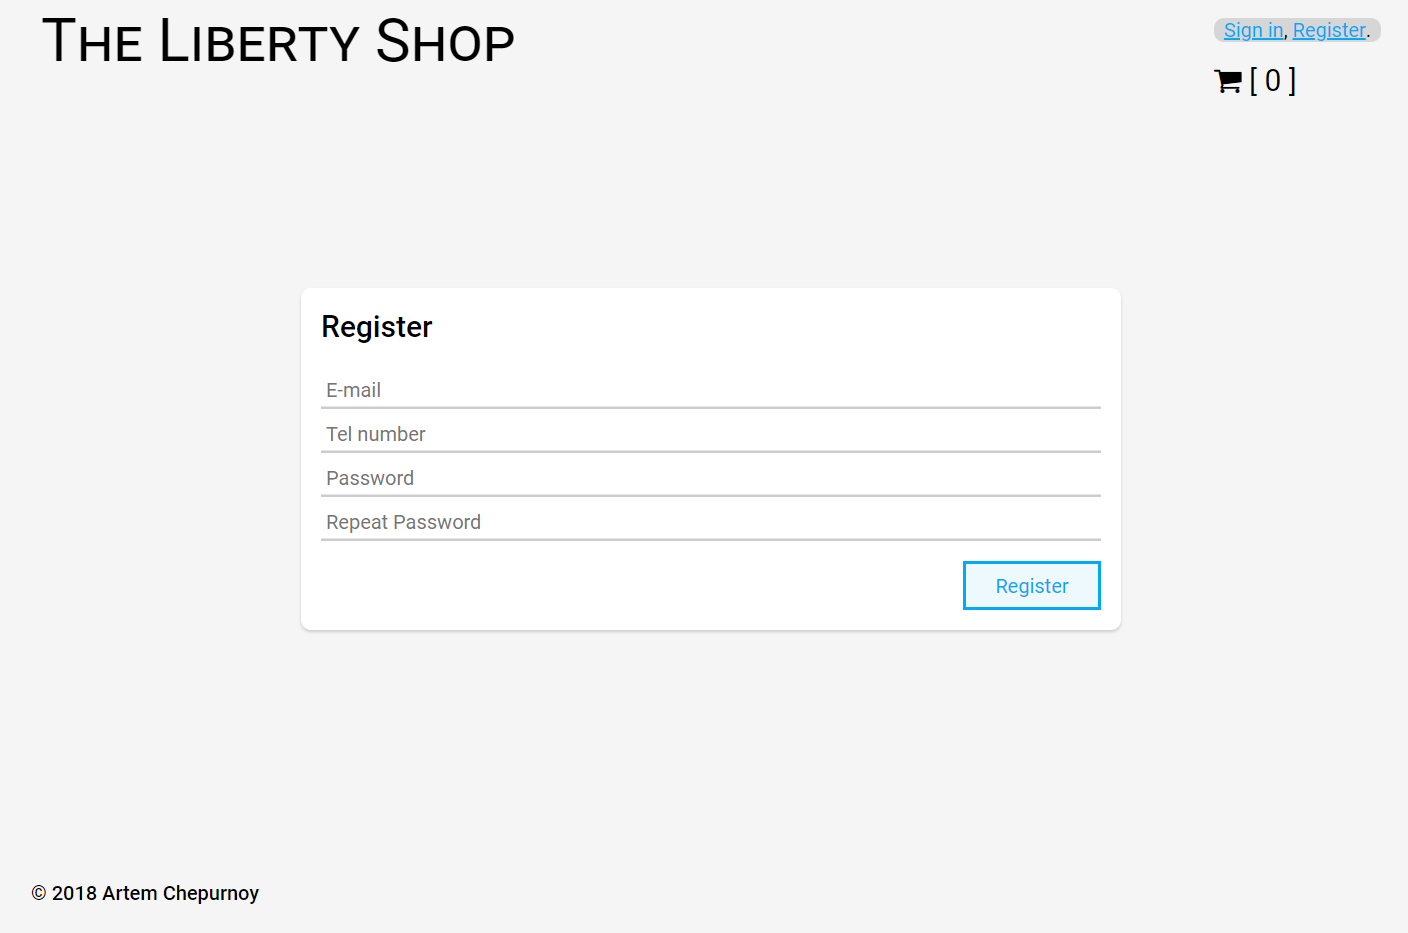
\includegraphics[width=0.8\textwidth]{screen_register}
    \caption{Сторінка реєстрації у системі}
    \label{fig:site_register}
\end{figure}

Після реєстрації користувач має увійти до системи~(рисунок~\ref{fig:site_login}).
\begin{figure}[H]
    \centering
    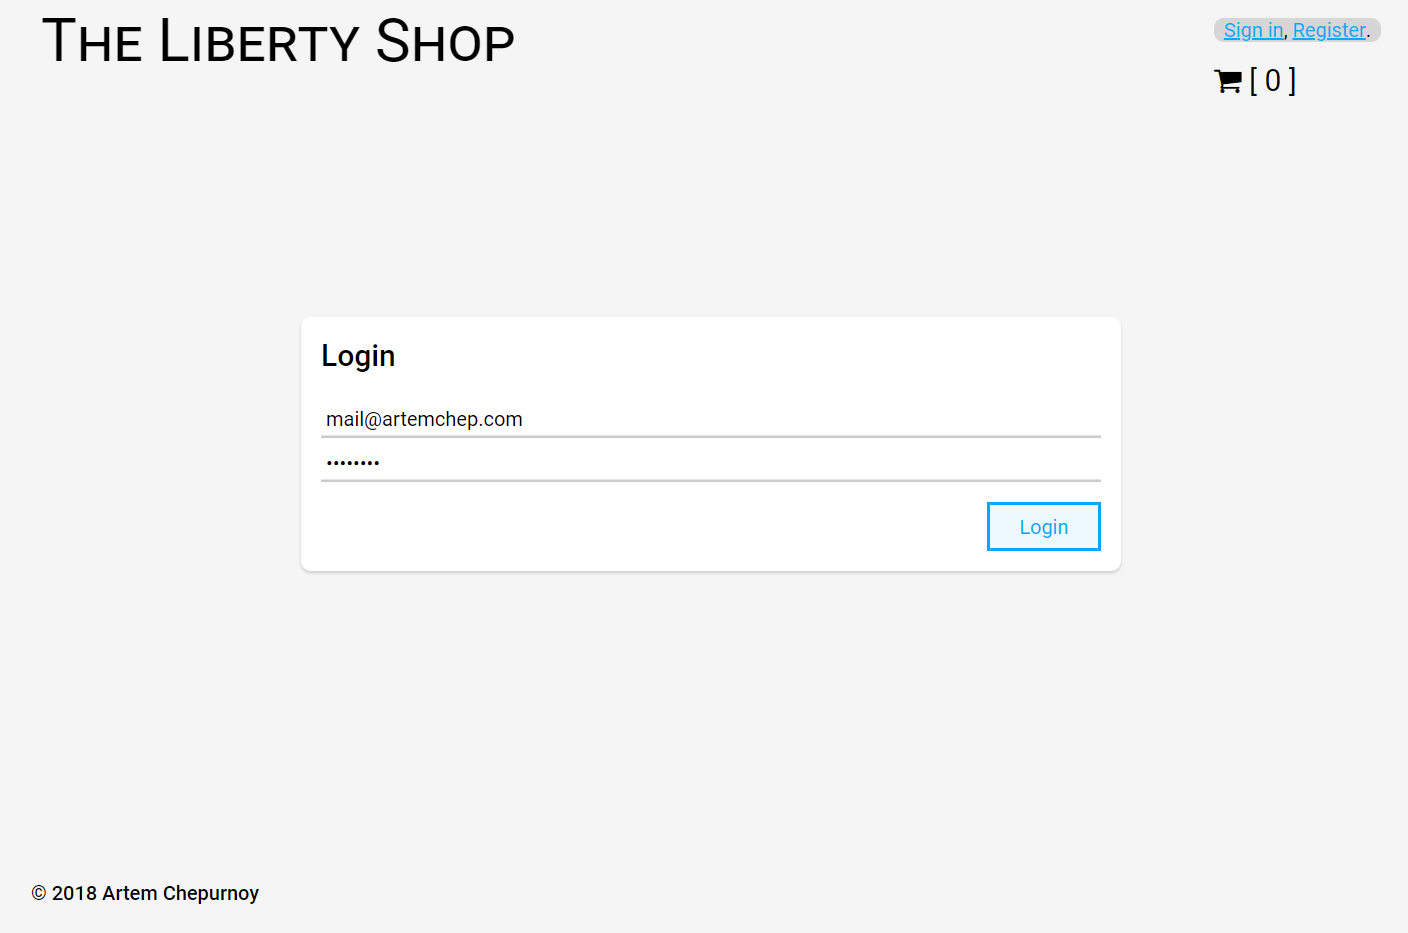
\includegraphics[width=0.8\textwidth]{screen_login}
    \caption{Сторінка входу до системи}
    \label{fig:site_login}
\end{figure}

Користувач може переглядати доступні товари на головній сторінці сайту.
Доступна можливість пошуку товару за ім'ям та категоріям.
\begin{figure}[H]
    \centering
    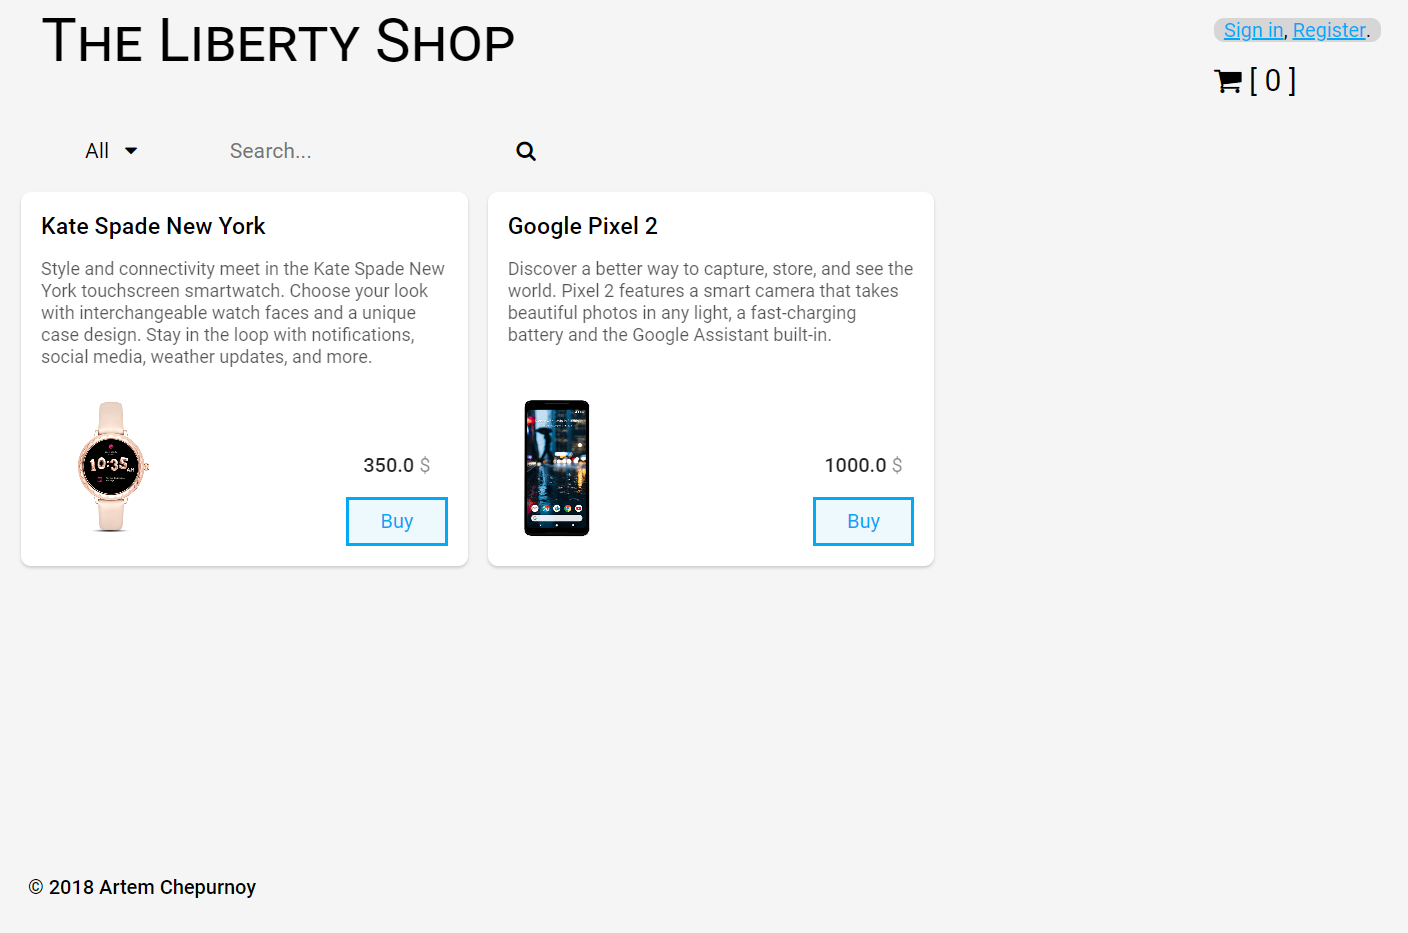
\includegraphics[width=0.8\textwidth]{screen_product__list}
    \caption{Головна сторінка ресурсу}
    \label{fig:site_product_list}
\end{figure}

Адміністратор та менеджери сайту мають на головній сторінці додаткові елементи~(рисунок~\ref{fig:site_product_list_admin}): 
\begin{itemize}
\item Кнопка редагування продуктів;
\item \textit{<<Add product>>} --- показати діалог додавання нового продукту;
\item \textit{<<Add category>>} --- показати діалог додавання нової категорії продуктів;
\item \textit{<<Edit category>>} --- показати діалог редагування та видалення категорії продуктів.
\end{itemize}
\begin{figure}[H]
    \centering
    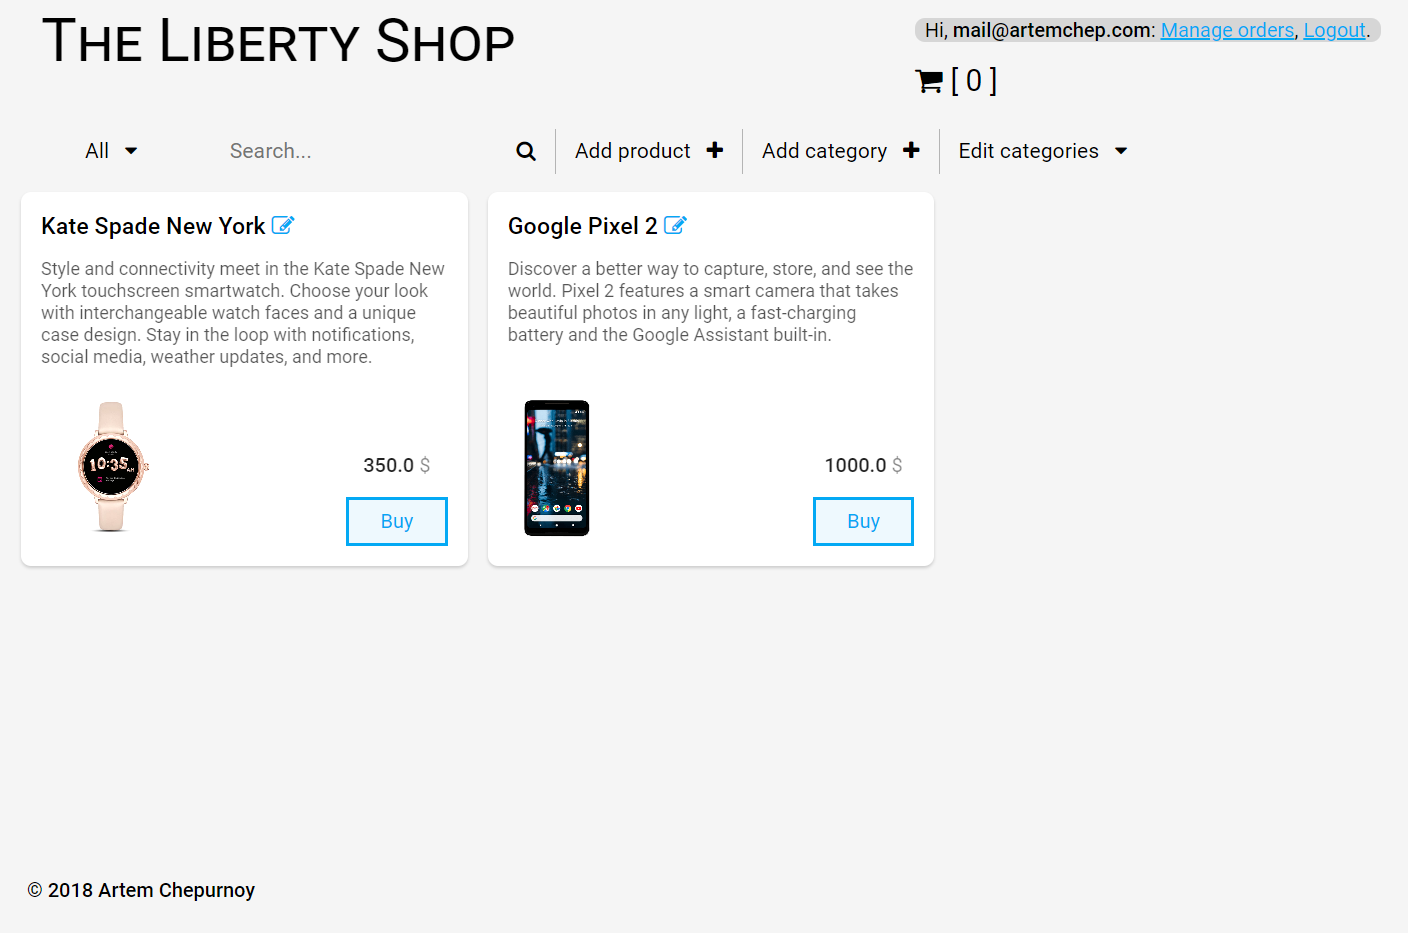
\includegraphics[width=0.8\textwidth]{screen_product__list__admin}
    \caption{Головна сторінка ресурсу (адміністратор)}
    \label{fig:site_product_list_admin}
\end{figure}

Діалог для створення нового продукту представлено на рисунку~\ref{fig:site_product_add}).

Продукт має такі властивості як категорія продуктів, назва, короткий опис, графічне зображення, ціна та розмірність.   
\begin{figure}[H]
    \centering
    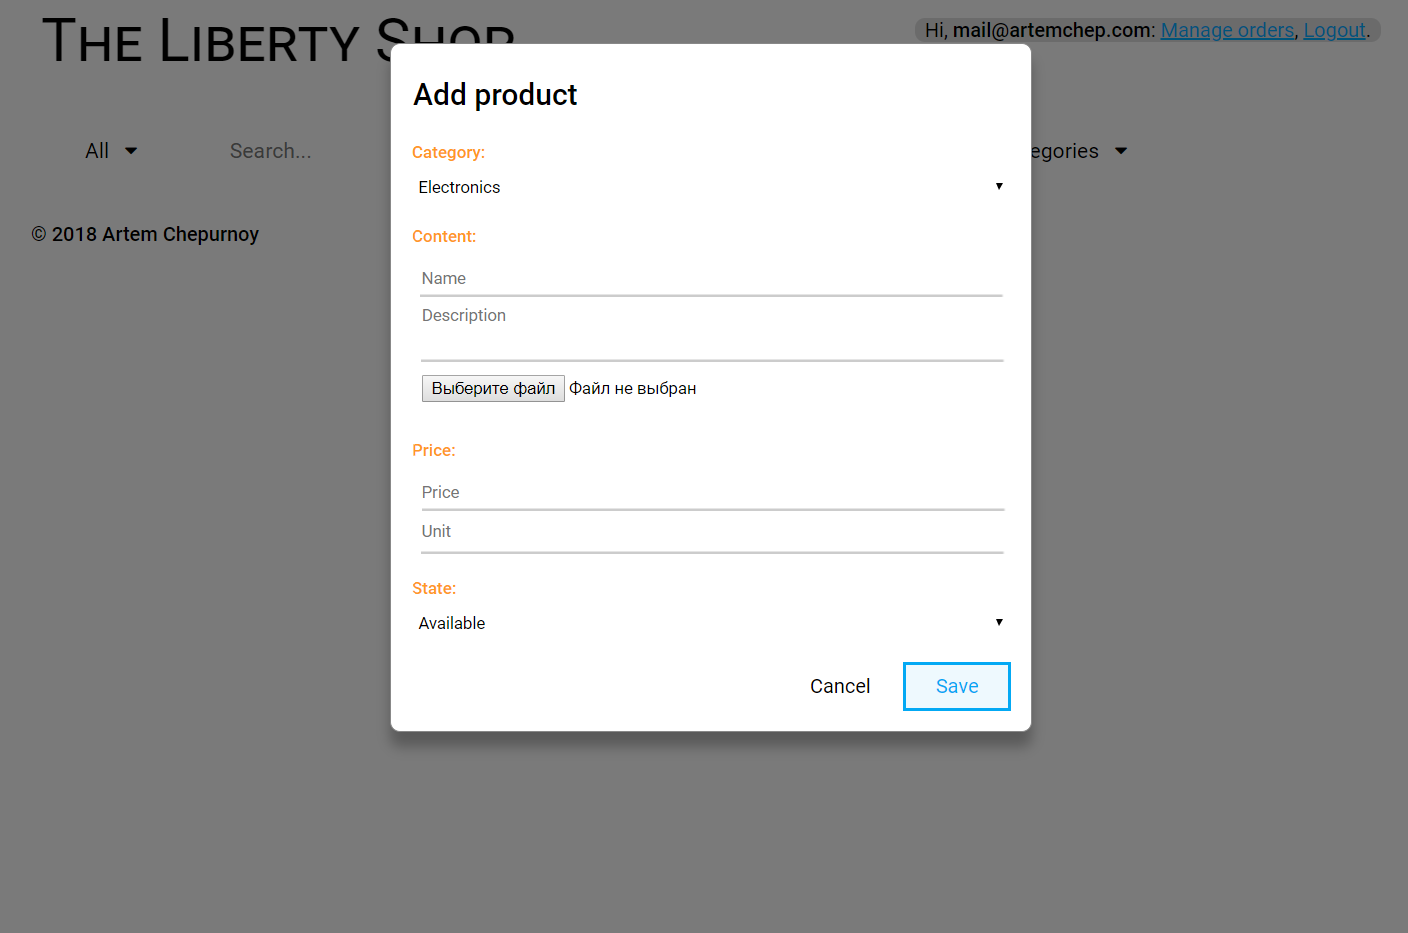
\includegraphics[width=0.8\textwidth]{screen_product_add}
    \caption{Діалог створення нового продукту}
    \label{fig:site_product_add}
\end{figure}

Адміністратор та менеджер ресурсу мають можливість переглянути список поточних або минулих замовлень~(рисунок~\ref{fig:site_order_list}), перемістити замовлення до архіву.
Є можливість фільтрування замовлень по даті створення, даті архівування, назві, категорії, кількості продуктів та ціні.   
\begin{figure}[H]
    \centering
    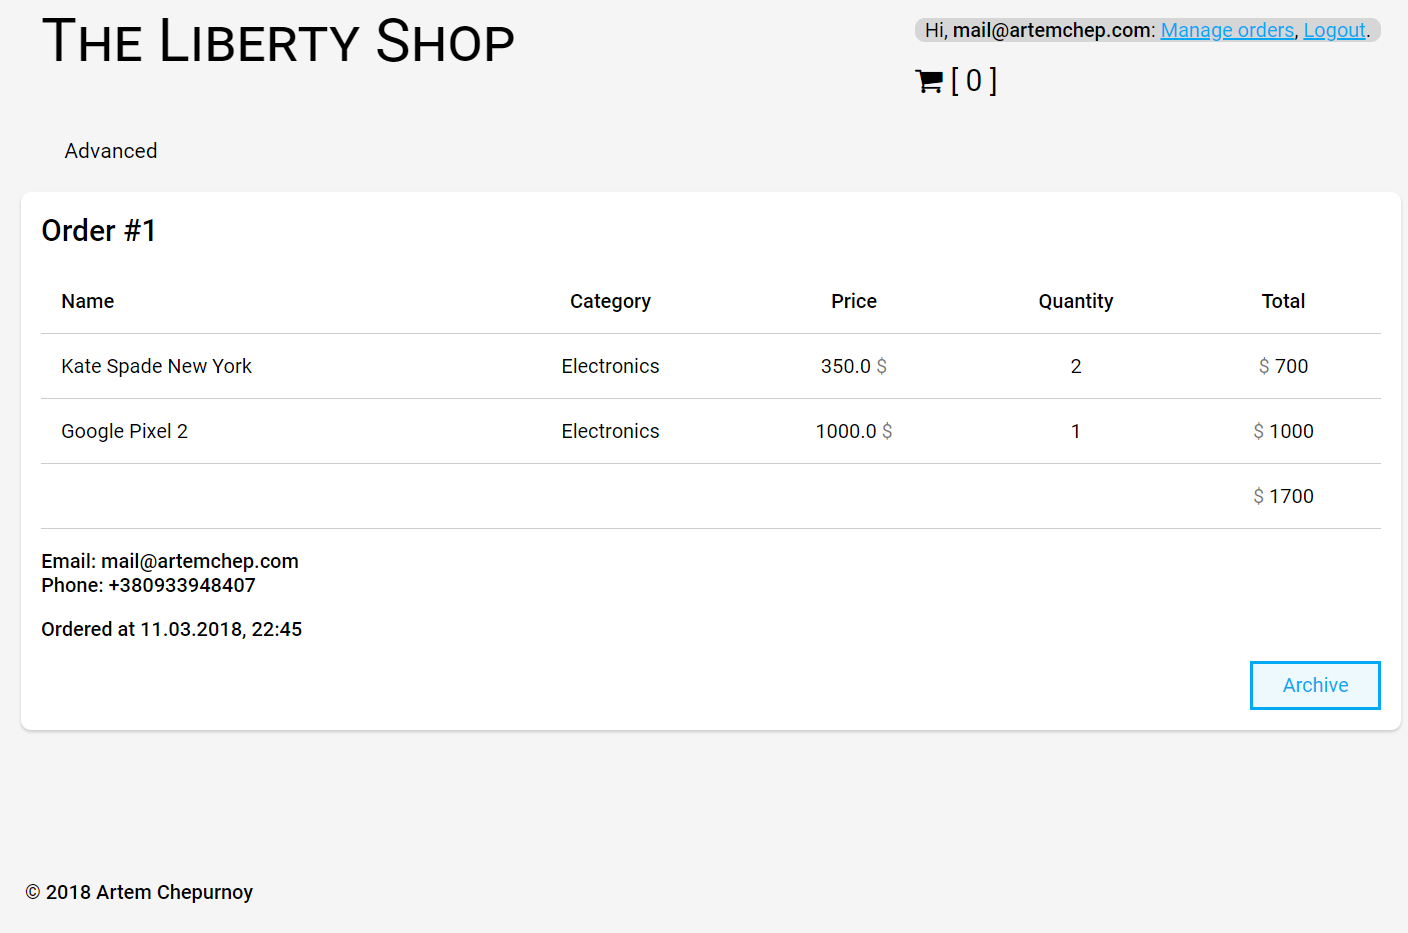
\includegraphics[width=0.8\textwidth]{screen_order__list}
    \caption{Сторінка керування замовленнями}
    \label{fig:site_order_list}
\end{figure}

\subsection{Результати тестування та рекомендації щодо удосконалення розробленої системи}
При тестуванні основною проблемою виявилася підтримка сайтом різних пристроїв та браузерів. 
При більш детальному вивченні стандартів HTML та CSS ця проблема була вирішена.

Одним із напрямків розвитку розробленої системи є співробітництво з іншими постачальниками, створення платформи для постачальників. 

\section{Програмна реалізація системи}
\subsection{Особливості програмної реалізації системи, що розробляється}
Для розробки програмної системи була використані мова програмування Kotlin та застосовані патерни проектування типу GoF.

Були застосовані принципи SOLID~\cite{Arch2007}:
\begin{enumerate}
	\item Принцип єдиного обов'язку --- принцип об'єктно-орієнтованого програмування, який означає, що клас має бути створений для виконання лише однієї задачі, яку він повинен повністю інкапсулювати.
	      Отже, всі сервіси цього класу мають бути повністю підпорядковані її виконанню.
	      Результатом слідування цій концепції є наявність лише однієї причини для зміни класу.
	\item Принцип відкритості/закритості --- принцип об'єктно-орієнтованого програмування, який означає, що програмні сутності, такі як класи, модулі, функції, методи та ін. мають бути <<відкритими для розширення та закритими для змін>>.
	      Це означає, що вони можуть надавати можливість змінювати свою поведінку без або з мінімальними змінами коду.
	\item Принцип заміщення Лісков --- якщо $S$ підтип $T$, тоді об'єкти типу $T$ в програмі можуть бути заміщені об'єктами типу $S$ без будь-яких змін бажаних властивостей цієї програми.
	\item Принцип розділення інтерфейсів --- принцип схожий із принципом єдиного обов'язку.
	      Застосування даного принципу полягає у розділі занадто <<товстих>> інтерфейсів на менші та специфічні, щоб їх клієнти знали лише про ті методи, що необхідні для них у роботі.
	      Як результат, при зміні певного функціоналу, незмінними мають лишитися ті класи, що не використовують його.
	      Тобто виконання цього принципу допомагає системі залишатися гнучкою при внесенні до неї змін та лишатися простою для рефакторингу.
	\item Принцип інверсії залежностей.
	      Принцип формулюється наступним чином: модулі вищого рівня не повинні залежати від модулів нижчого рівня, обидва типи модулів повинні залежати від абстракцій; абстракції не повинні залежати від деталей реалізації, деталі реалізації повинні залежати від абстракцій.
\end{enumerate}

Система реалізована у парадігмі чистої архітектури, яка полягає в розділенні системи на 3 рівні~\cite{Arch2007}:
\begin{enumerate}
	\item Рівень даних --- рівень даних у чистому вигляді, що складається з сутностей, які є основними бізнес-правилами системи.
	\item Доменний рівень --- рівень бізнес-логіки додатку, що відповідає за основний функціонал системи, її поведінку та правила, що стосуються конкретного додатку.
	\item Рівень представлення --- рівень користувацького інтерфейсу, відображення даних, обробки користувацьких подій.
\end{enumerate}

\subsection{Тестування програмного забезпечення}
\subsubsection{Загальна теорія тестування}
Тестування --- перевірка відповідності реальної поведінки програми очікуваній, що здійснюється на кінцевому наборі тестів, який був обраний певним чином.
У більш широкому сенсі, тестування --- це одна з технік контролю якості, що включає в себе активності з планування робіт, проектування тестів, виконання тестування і аналізу отриманих результатів~\cite{Swebok}.

Верифікація --- це процес оцінки системи або її компонентів з метою визначення чи задовольняють результати поточного етапу розробки умовам, що були сформовані на початку цього етапу.
Тобто чи виконуються наші цілі, терміни, завдання по розробці проекту, визначені на початку поточної фази~\cite{Swebok}.

Валідація --- це визначення відповідності ПО, що розроблюється очікуванням і потребам користувача, вимогам до системи~\cite{Swebok}.

\subsubsection{Тестування програмної системи}
На першому етапі тестування необхідно провести модульне тестування усіх компонентів системи, які можуть бути протестовані окремо від інших у штучному середовищі тестування.
Для Unit-тестування використовується засоб автоматизації тестування Kotest.

Такий вибір зумовлений простотою інтеграції з Kotlin.
Kotest надає великий об'єм валідаційних методів, завдяки яким можна легко та ефективно тестувати як модулі обробки даних та взаємодії з базами даних, так і модулі вводу та виводу інформації~\cite{Kotest}.

Фрагмент застосованих Kotest тестів для валідації коректної роботи класу \texttt{GlobeHipster} приведено нижче:
\lstinputlisting{code/tests.kt}

\subsection{Інтерфейс програмного забезпечення}
Розроблена програмна система має консольний інтерфейс. Для запуску моделювання необхідно виконати такі команди:
\begin{lstlisting}
> jar kagent.jar --period=14 --time=5 configuration_a.json configuration_b.json
\end{lstlisting}
\begin{description}
	\item[де] \texttt{kagent.jar} --- назва бінарного файла програмної системи;
	\item \texttt{--period=14} --- період поповнення запасів регіональними та національними складами, у днях;
	\item \texttt{--time=5} --- час моделювання системи, у секундах;
	\item \texttt{configuration\_a.json} --- шлях до файлу конфігурації першого варіанта логістичної системи;
	\item \texttt{configuration\_b.json} --- шлях до файлу конфігурації другого варіанта логістичної системи.
\end{description}

В процесі моделювання логістичної системи у консоль виводиться поточний стан логістичної системи.
Фрагмент логування початкової загрузки конфігурації логістичної системи:
\begin{lstlisting}
Connecting Киев to Пирятин by 154.0 km. road
Connecting Житомир to Винница by 127.0 km. road
Connecting Николаев to Мелитополь by 299.0 km. road
Connecting Николаев to Саки by 325.0 km. road
Connecting Днепропетровск to Днепродзержинск by 45.0 km. road
Connecting Львов to Дубляны by 9.0 km. road
\end{lstlisting}

Фрагмент логування процесу моделювання логістичної системи:
\begin{lstlisting}
[432]
.     Current time is 432 days.
.    service level is 87%.
. avg. stock level is 92%.
[433]
.     Current time is 433 days.
.    service level is 88%.
. avg. stock level is 92%.
[434]
.     Current time is 434 days.
.    service level is 88%.
. avg. stock level is 91%.
\end{lstlisting}

Для генерації дампу поточного стану системи у файл необхідно натиснути клавішу <<S>> під час процесу моделювання, для призупинення виконування програми необхідно натиснути клавішу <<P>>.
Графічний інтерфейс складається з двох частин: меню та панелі поточного стану моделі.

Після закінчення часу на моделювання системи показується окно з динамікою зміни рівня сервісу за час моделювання (рисунок~\ref{fig:graph_sample}).

\begin{figure}[H]
	\centering
	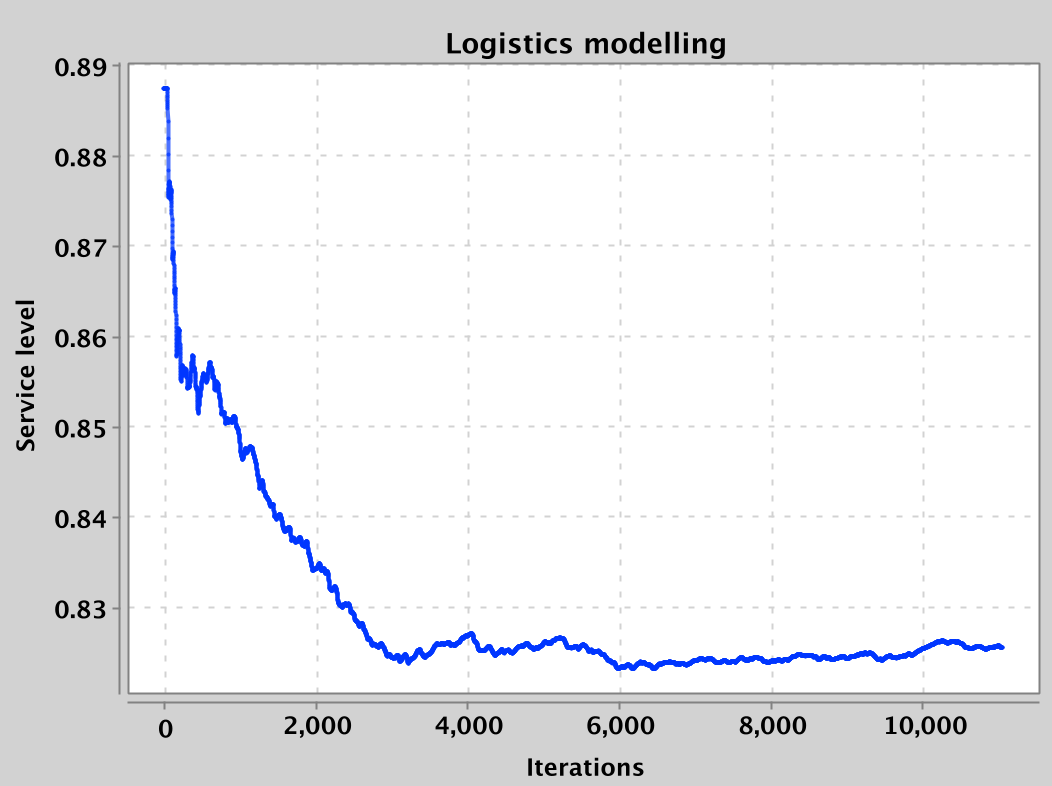
\includegraphics[width=0.6\textwidth]{graph_sample}
	\caption{Динаміка зміни рівня сервісу}
	\label{fig:graph_sample}
\end{figure}

\subsection{Аналіз продуктивності програмного забезпечення}
Розроблений програмний продукт широко використовує паралельні обчислення. 
В якості основи для паралельних обчислень було використано технологію Kotlin coroutines.

Для порівняння роботи програми у багатопотоковому режимі та однопотоковому режимі був проведений експеримент: моделювання логістичної системи~\cite{Годлевський2019} з обмеженої кількістю агентів на регіональному шару. Результат експерименту представлено на рисунку~\ref{fig:performance}.

\begin{figure}[H]
	\centering
	\begin{tikzpicture}
		\begin{axis}[
				scaled y ticks = false,
				xlabel={Кількість кінцевих споживачів продукції},
				xlabel near ticks,
				ylabel={Ітерацій за 100 мілісекунд},
				ylabel near ticks,
				ymajorgrids=true,
				line width=0.4mm,
				grid style=dashed,
			]
			\addplot table [x=n, y=i] {data/test_cpu.csv};
			\addplot table [x=n, y=z] {data/test_cpu.csv};
			\legend{багатопотоковий режим,однопотоковий режим}
		\end{axis}
	\end{tikzpicture}
	\caption{Результати оцінки продуктивності~\acrshort{sw}}
	\label{fig:performance}
\end{figure}

Програмний продукт у багатопотоковому режимі працює в $\~5$ разів швидше ніж у однопотоковому режимі. 
Це обумовлено тим що експеримент проводився на комп'ютері з чотирма ядрами процессору і у многопоточному режимі програма використовує всі ресурси всіх процесорів, а в однопотоковому режимі тільки один.  

\subsection{Аналіз результатів дослідження}
Початкова конфігурація була взята з роботи~\cite{Годлевський2019} яка в свою чергу базується на роботі <<Моделі і інформаційна технологія стратегічного управління логістичною системою дистрибуції>>~\cite{Stankevich}.

З метою формування множини ефективних рішень конфігурації логістичної системи в роботі були приведені прорахунки для двох варіантів базового рівня сервісу на регіональних складах: $84.13\%$, $97.72\%$. Для кожного базового рівня сервісу розглядалися тривалості циклів замовлень з виробничого на національний і далі на регіональний рівні: 2, 3 і 4 тижні.

Таким чином було сформовано 36 конфігурацій логістичних мереж, для кожної з котрих було проведено моделювання рівня сервісу.

Результати експерименту приведені в таблиці~\ref{tab:results}.

{
\small
\tabulinesep=1.2mm
\begin{longtabu} to \textwidth {|X[1,c]|X[1,c]|X[1,c]|X[1,c]|X[1,c]|}
	\caption{Результати експерименту моделювання конфігурацій логістичних систем}
	\label{tab:results} \\
	\hline
	Кількість регіональних складів & Тривалість циклу, тижнів & Базовий рівень страхового запасу, \% & Сумарні логістичні витрати~\cite{Годлевський2019} & Мережевий рівень сервісу \\
	\hline
	\endfirsthead
	\caption*{Закінчення таблиці \thetable{}}\\
	\hline
	Кількість регіональних складів & Тривалість циклу, тижнів & Базовий рівень страхового запасу, \% & Сумарні логістичні витрати~\cite{Годлевський2019} & Мережевий рівень сервісу \\
	\hline
	\endhead
	5 & \multirow{4}{*}{2} & \multirow{12}{*}{$84.13$} & $183729.3882$ & $0.864868$ \\ \cline{1-1}\cline{4-5}
	6 & & & $185253.5535$ & $0.868993$ \\ \cline{1-1}\cline{4-5}
	7 & & & $185649.9391$ & $0.871659$ \\ \cline{1-1}\cline{4-5}
	8 & & & $185935.0956$ & $0.873573$ \\ \cline{1-2}\cline{4-5}

	5 & \multirow{4}{*}{3} & & $195332.5978$ & $0.830533$ \\ \cline{1-1}\cline{4-5}
	6 & & & $196856.7631$ & $0.831683$ \\ \cline{1-1}\cline{4-5}
	7 & & & $197253.1487$ & $0.831786$ \\ \cline{1-1}\cline{4-5}
	8 & & & $197538.3052$ & $97$ \\ \cline{1-2}\cline{4-5}

	5 & \multirow{4}{*}{4} & & $206935.8074$ & $0.793313$ \\ \cline{1-1}\cline{4-5}
	6 & & & $208459.9727$ & $0.800558$ \\ \cline{1-1}\cline{4-5}
	7 & & & $208856.3583$ & $0.804958$ \\ \cline{1-1}\cline{4-5}
	8 & & & $209141.5148$ & $0.808666$ \\ \hline

	5 & \multirow{4}{*}{2} & \multirow{12}{*}{$97.72$} & $187478.0538$ & $0.931035$ \\ \cline{1-1}\cline{4-5}
	6 & & & $189002.2191$ & $0.938148$ \\ \cline{1-1}\cline{4-5}
	7 & & & $189398.6047$ & $0.939289$ \\ \cline{1-1}\cline{4-5}
	8 & & & $189683.7612$ & $0.940954$ \\ \cline{1-2}\cline{4-5}

	5 & \multirow{4}{*}{3} & & $200955.5962$ & $0.895327$ \\ \cline{1-1}\cline{4-5}
	6 & & & $202479.7615$ & $0.896253$ \\ \cline{1-1}\cline{4-5}
	7 & & & $202876.1471$ & $0.898870$ \\ \cline{1-1}\cline{4-5}
	8 & & & $203161.3036$ & $0.900588$ \\ \cline{1-2}\cline{4-5}

	5 & \multirow{4}{*}{4} & & $214433.1386$ & $0.859070$ \\ \cline{1-1}\cline{4-5}
	6 & & & $215957.3039$ & $0.867487$ \\ \cline{1-1}\cline{4-5}
	7 & & & $216353.6895$ & $0.870390$ \\ \cline{1-1}\cline{4-5}
	8 & & & $216638.846$ & $0.877827$ \\ \hline
\end{longtabu}
}

Візуалізація зміни рівня сервісу представлені на рисунках~\ref{fig:graph_84},~\ref{fig:graph_99}.

\begin{figure}[H]
	% \def\axisdefaultwidth{14cm}
	% \def\axisdefaultheight{10сm}
	\centering
	\begin{tikzpicture}
		\begin{axis}[
				legend style={font=\footnotesize,at={(1.6,1.0)},anchor=north east},
				xmin=0,
				xmax=10000,
				xlabel={Номер ітерації моделювання},
				xlabel style={yshift=-1cm},
				ylabel={Рівень сервісу},
				ylabel near ticks,
				ymajorgrids=true,
				grid style=dashed,
				line width=0.4mm,
				mark size=0pt,
				mark = none,
				smooth
			]
			\addplot table [x=i, y=1] {data/dynamic_84.csv};
			\addplot table [x=i, y=2] {data/dynamic_84.csv};
			\addplot table [x=i, y=3] {data/dynamic_84.csv};
			\addplot table [x=i, y=4] {data/dynamic_84.csv};
			\addplot table [x=i, y=5] {data/dynamic_84.csv};
			\addplot table [x=i, y=6] {data/dynamic_84.csv};
			\addplot table [x=i, y=7] {data/dynamic_84.csv};
			\addplot table [x=i, y=8] {data/dynamic_84.csv};
			\addplot table [x=i, y=9] {data/dynamic_84.csv};
			\addplot table [x=i, y=10] {data/dynamic_84.csv};
			\addplot table [x=i, y=11] {data/dynamic_84.csv};
			\addplot table [x=i, y=12] {data/dynamic_84.csv};
			\legend{5 складів; 2 тижня,6 складів; 2 тижня,7 складів; 2 тижня,8 складів; 2 тижня,5 складів; 3 тижня,6 складів; 3 тижня,7 складів; 3 тижня,8 складів; 3 тижня,5 складів; 4 тижня,6 складів; 4 тижня,7 складів; 4 тижня,8 складів; 4 тижня}
		\end{axis}
	\end{tikzpicture}
	% 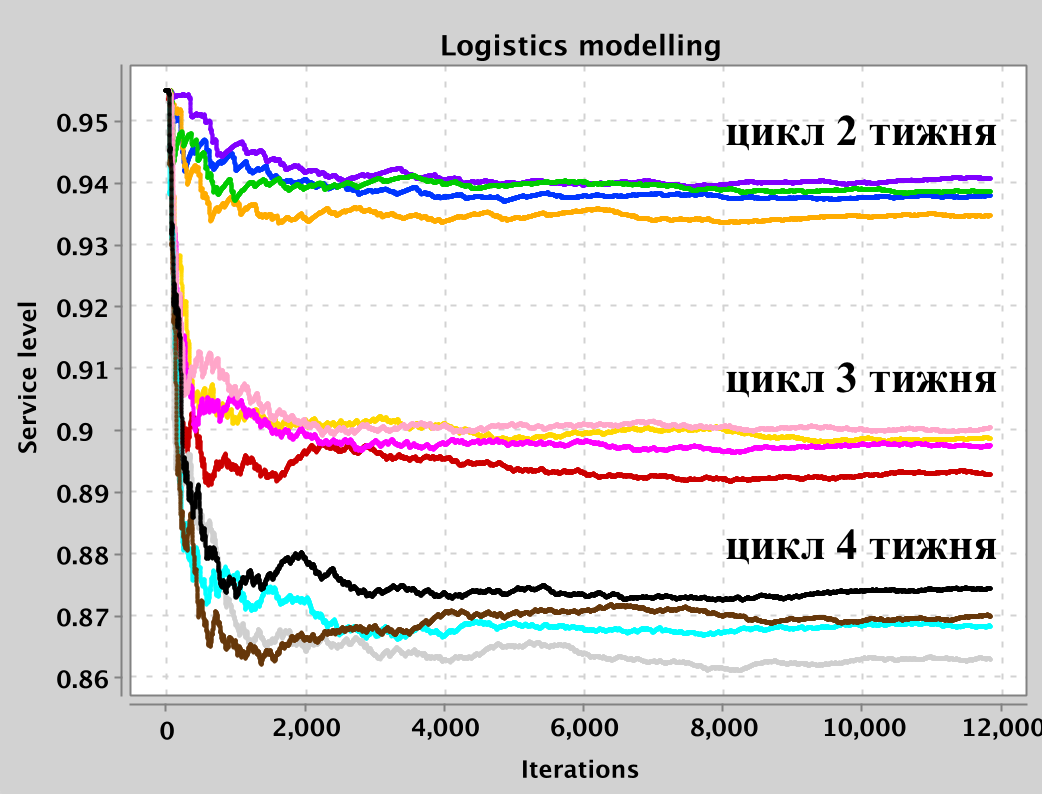
\includegraphics[width=0.6\textwidth]{graph_99}
	\caption{Динаміка зміни рівня сервісу для групи конфігурацій з базовим рівнем страхового запасу рівним $84.13$}
	\label{fig:graph_84}
\end{figure}

\begin{figure}[H]
	% \def\axisdefaultwidth{14cm}
	% \def\axisdefaultheight{10сm}
	\centering
	\begin{tikzpicture}
		\begin{axis}[
				legend style={font=\footnotesize,at={(1.6,1.0)},anchor=north east},
				xmin=0,
				xmax=10000,
				xlabel={Номер ітерації моделювання},
				xlabel style={yshift=-1cm},
				ylabel={Рівень сервісу},
				ylabel near ticks,
				ymajorgrids=true,
				grid style=dashed,
				line width=0.4mm,
				mark size=0pt,
				mark = none,
				smooth
			]
			\addplot table [x=i, y=1] {data/dynamic_97.csv};
			\addplot table [x=i, y=2] {data/dynamic_97.csv};
			\addplot table [x=i, y=3] {data/dynamic_97.csv};
			\addplot table [x=i, y=4] {data/dynamic_97.csv};
			\addplot table [x=i, y=5] {data/dynamic_97.csv};
			\addplot table [x=i, y=6] {data/dynamic_97.csv};
			\addplot table [x=i, y=7] {data/dynamic_97.csv};
			\addplot table [x=i, y=8] {data/dynamic_97.csv};
			\addplot table [x=i, y=9] {data/dynamic_97.csv};
			\addplot table [x=i, y=10] {data/dynamic_97.csv};
			\addplot table [x=i, y=11] {data/dynamic_97.csv};
			\addplot table [x=i, y=12] {data/dynamic_97.csv};
			\legend{5 складів; 2 тижня,6 складів; 2 тижня,7 складів; 2 тижня,8 складів; 2 тижня,5 складів; 3 тижня,6 складів; 3 тижня,7 складів; 3 тижня,8 складів; 3 тижня,5 складів; 4 тижня,6 складів; 4 тижня,7 складів; 4 тижня,8 складів; 4 тижня}
		\end{axis}
	\end{tikzpicture}
	% 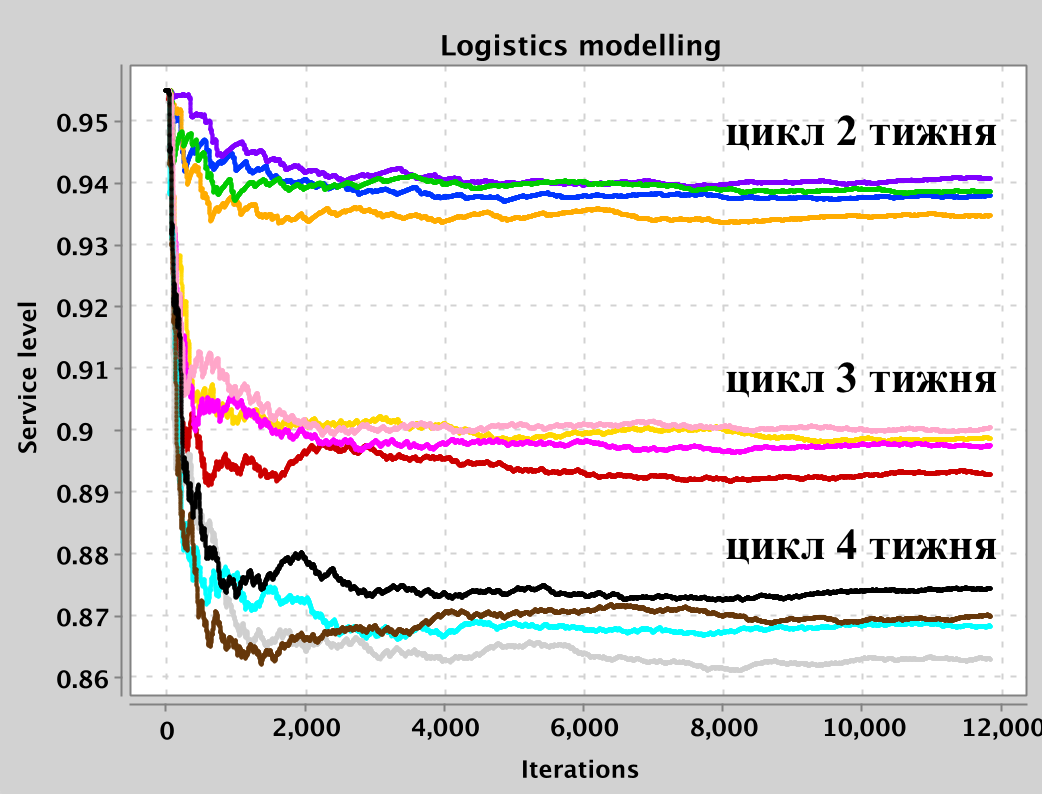
\includegraphics[width=0.6\textwidth]{graph_99}
	\caption{Динаміка зміни рівня сервісу для групи конфігурацій з базовим рівнем страхового запасу рівним $97.72$}
	\label{fig:graph_99}
\end{figure}

Наглядна графічна інтерпретація результатів з таблиці~\ref{tab:results} зображена на рисунку~\ref{fig:results}.

\begin{figure}[H]
	\centering
	\begin{tikzpicture}
		\begin{axis}[
				scaled y ticks = false,
				xlabel={Сумарні логістичні витрати},
				xlabel style={yshift=-1cm},
				ylabel={Мережевий рівень сервісу},
				ylabel near ticks,
				enlargelimits=false,
				line width=0.4mm,
				ymajorgrids=true,
				grid style=dashed,
			]
			\addplot+[
				only marks,
				scatter,
				mark=halfcircle*,
				mark size=2.9pt]
			table[meta=y]
				{data/results.csv};
		\end{axis}
	\end{tikzpicture}
	\caption{Результати експерименту моделювання конфігурацій логістичних систем}
	\label{fig:results}
\end{figure}

Проведемо аналіз отриманих результатів.
Незалежно від тривалості циклів замовлень рівень сервісу збільшується зі збільшенням кількості регіональних складів.
Це можна пояснити тим, що збільшується загальний розмір страхових запасів.
Мережевий рівень сервісу зменшується зі збільшенням тривалості циклів замовлень. Це пов'язано з тим, що при меншому циклі замовлень є більше можливостей на адаптацію до змін попиту.
Зі збільшенням базового рівня сервісу збільшується рівень мережевого сервісу.
Виходячи з проведеного аналізу, можна зробити висновок, що безліч ефективних рішень знаходиться в лівому верхньому кутку графіка (рис.~\ref{fig:results}). Залежно від пріоритету експерту по відношенню до критеріїв: сумарні логістичні витрати, мережевий рівень сервісу вибирається прийнятна конфігурація логістичної системи.

Подальше використання отриманих результатів пов'язане з визначенням стійкості рівня сервісу до різноманітних надзвичайних ситуацій. Отримані результати є основою для формування організаційної структури управління логістичною системою дистрибуції.

\section*{Висновки}
\addcontentsline{toc}{section}{Висновки}
Сучасні алгоритми <<комп'юторного зору>> дозволяють досить швидко створювати вражаючі програми які реалізують зоровий інтерфейс.
Використання нейронних мереж спрощує задачу переведення точок обличчя у положення погляду не екрані.

В ході написання роботи дану задачу було розкрито повною мірою на прикладі проектування та реалізації програмної системи для визначення погляду користувача з видеоряду та керування курсором за допомогою погляду. 

В процесі дослідження були сформульовані вимоги до програмної системи, та обрана й спроектована її архітектура.
Обгрунтований вибір інструментальних засобів розробки.

\printbibliography[heading=bibintoc, title={Список джерел інформації}]


\end{document}